\subsection{Bolivia}\label{subsec:bol}

Three WCD are operating, since 2009, at the cosmic ray laboratory on mount
Chacaltaya, near the city of La Paz, Bolivia. The high elevation of the
laboratory (see table \ref{tab:locations}) improves the sensitivity of a WCD to
low energy showers with respect to a WCD with similar characteristics operating
at sea level.

Each of the WCD operating on mount Chacaltaya has a volume of pure water
contained in a cylindrical tank made of either plastic or fiberglass. The
volume of water is observed from above by an 8"  Electron Tubes
photomultiplier that collects Cherenkov photons emitted by the medium when
charged particles hit the detector. Moreover, the water has been
mixed with Amino-G, a chemical compound that acts as a wave length shifter,
thus effectively increasing the number of photons collected by the
photomultiplier. The walls of each tank are internally covered with a
reflective liner to improve the collection efficiency of the detector. Two
different materials were used as reflective liners, and their reflection
coefficients have been measured employing a violet led. Table \ref{tab:chars}
contains some of the characteristics for each of the WCDs operating at the
laboratory including the reflection coefficient. The configuration of the WCD
at the laboratory is sketched in the left side of figure \ref{fig:bolivia-wcd},
while the right side shows a picture of one the assembled detectors.

\begin{figure}[h!]
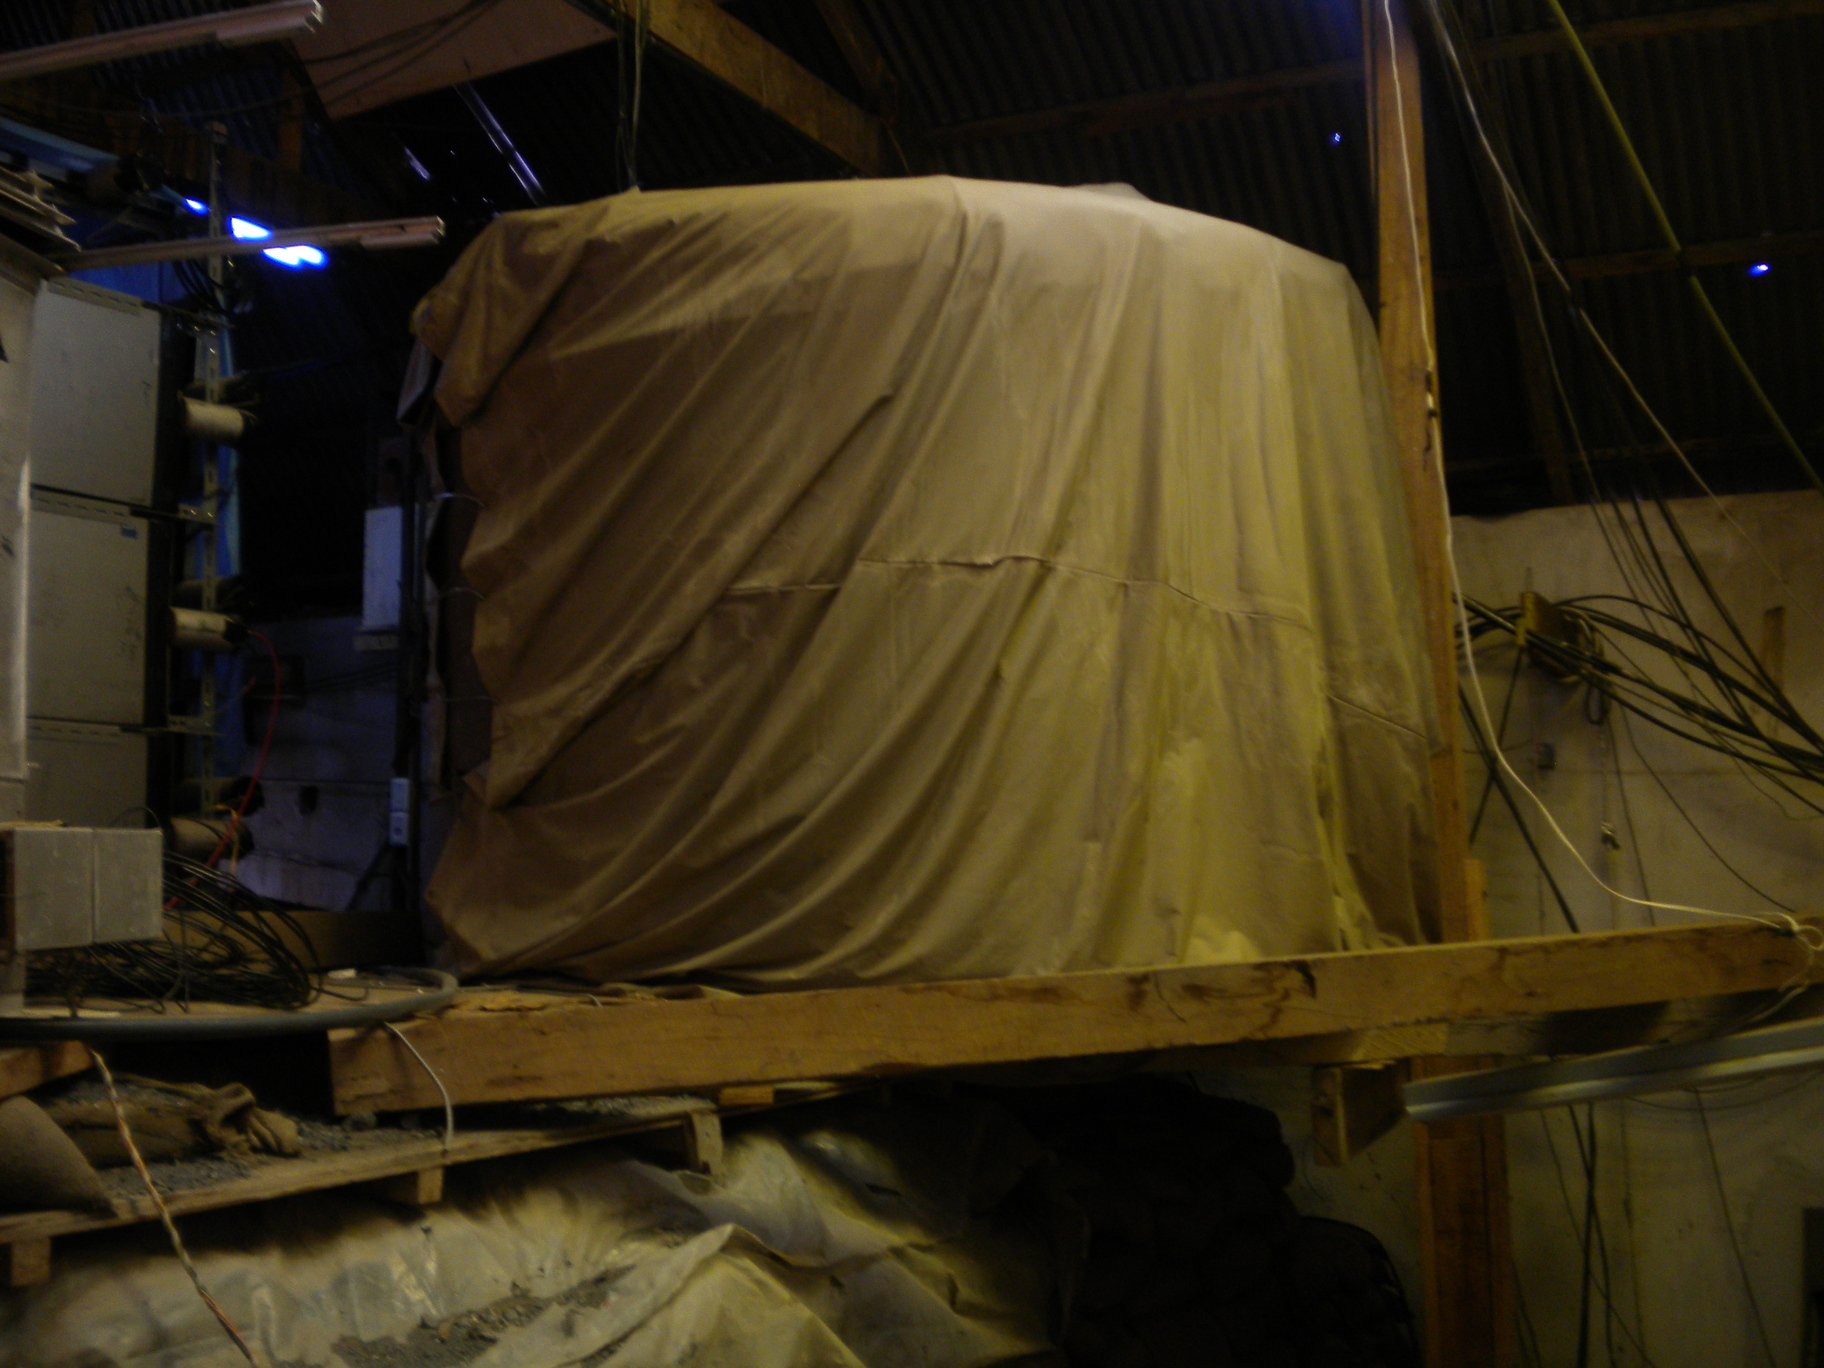
\includegraphics[width=0.5\textwidth]{images/bolivia/cha1139-m.jpg}
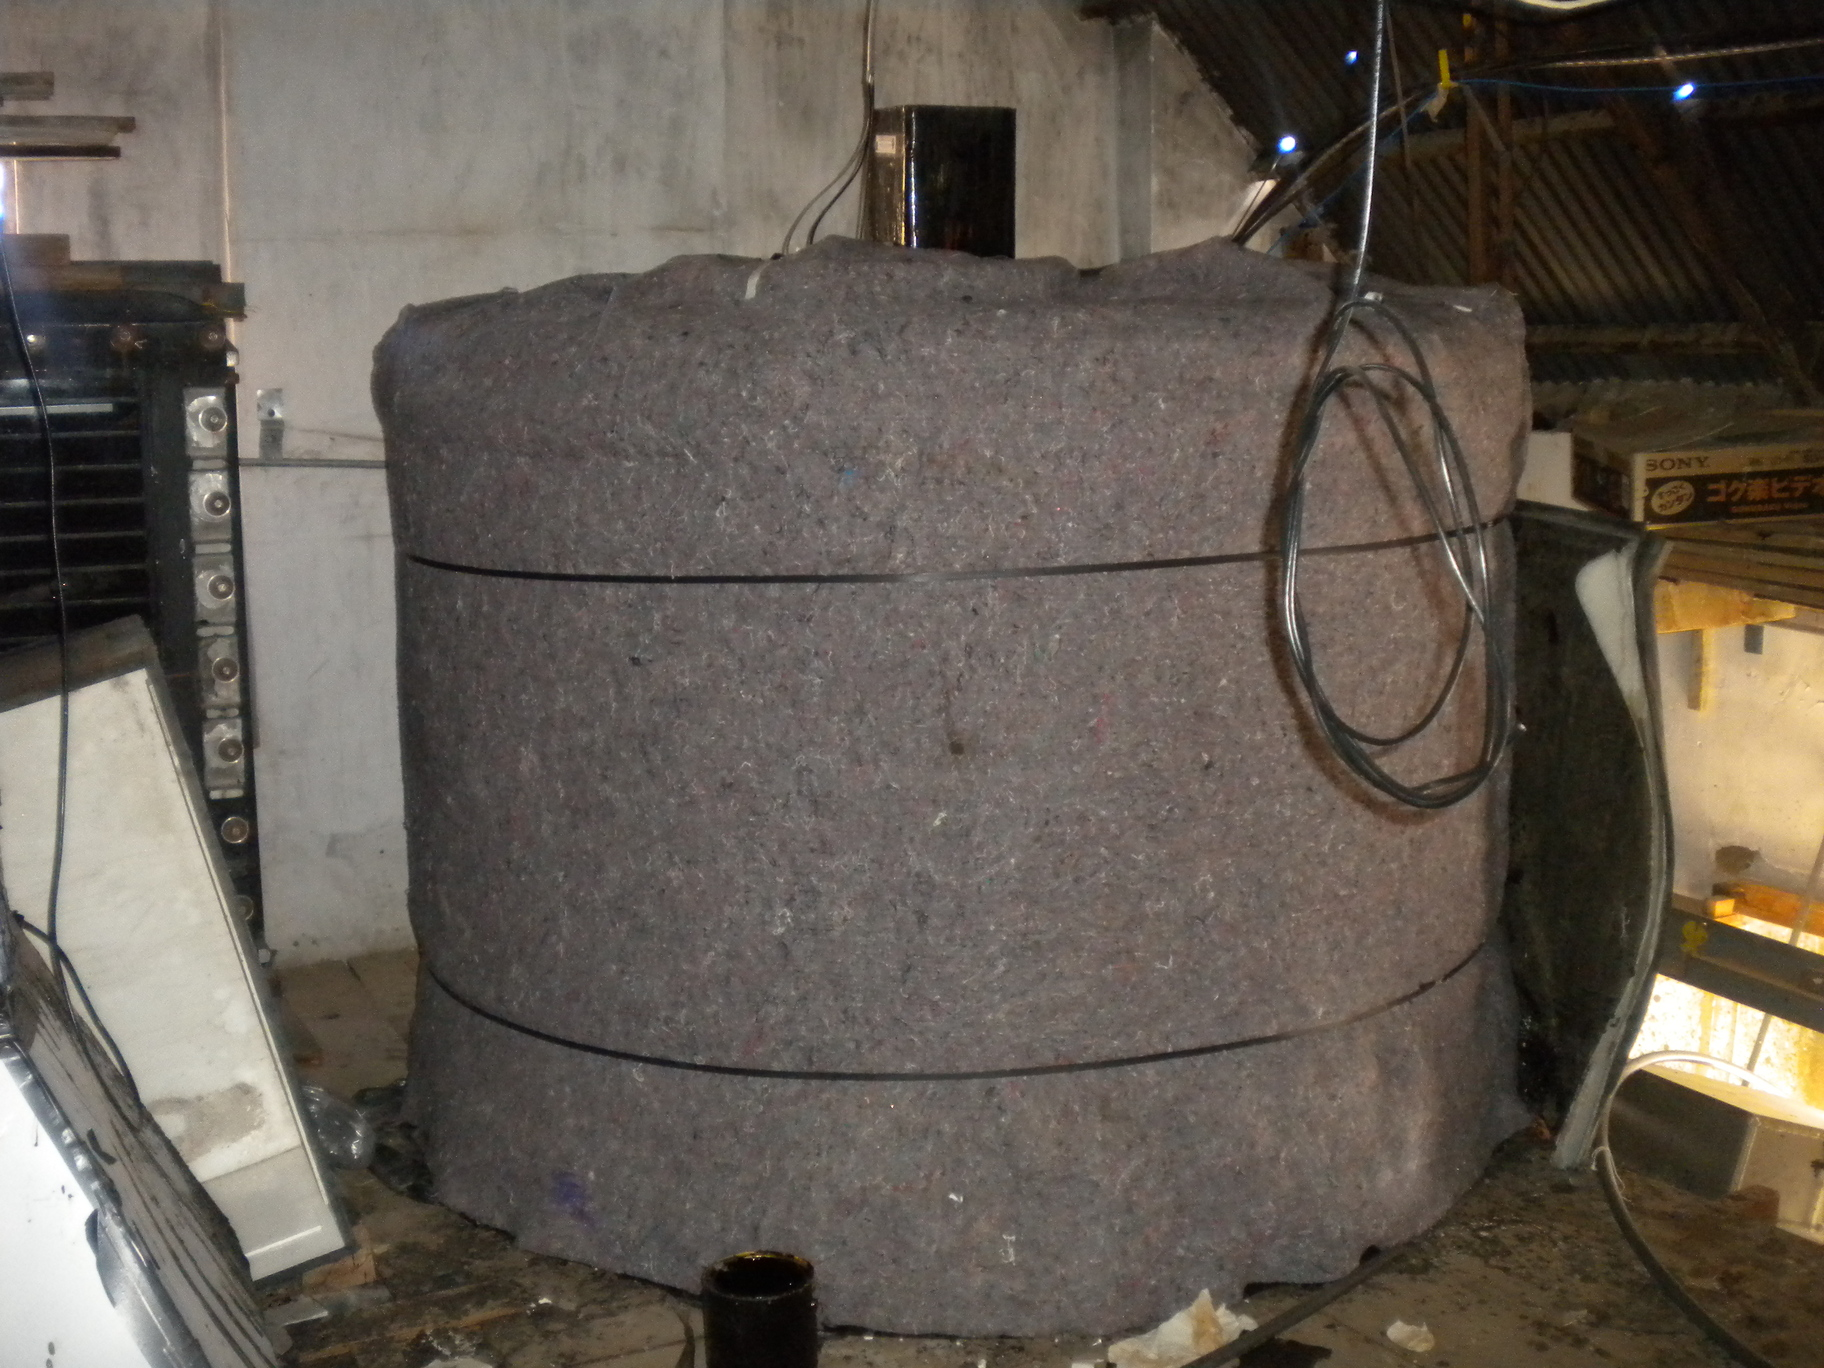
\includegraphics[width=0.5\textwidth]{images/bolivia/cha1140-m.jpg}
\caption{Pictures of two of the three WCD installed in mount Chacaltaya.}
\label{fig:bolivia-wcd}
\end{figure}

\begin{table}
\begin{center}
\begin{tabular}{|c|c|c|}
\hline
	& WCD1 & WCD2 \& WCD3\\
\hline
Diameter & $1.4\ \rm{m}$ & $2.2\ \rm{m}$\\
Water depth & $1.4\ \rm{m}$ & $1.5\ \rm{m}$\\
Water volume & $2200\ \rm{l}$ & $5300\ \rm{l}$\\
Amino G & yes & only in WCD2\\
Tank material & plastic & fiberglass\\
Liner material & Tyvek\textregistered & vinyl\\
Liner reflection coefficient & 0.8 & 0.9\\
Photomultiplier & 9353KB 8" & 9353KB 8"\\
\hline
\end{tabular}
\caption{Relevant characteristics of each WCD operating on mount Chacaltaya.}
\label{tab:chars}
\end{center}
\end{table}

Data acquisition is performed by means of a local station (LS), designed and
implemented at the Centro Atómico Bariloche, based on the data acquisition
electronics from the Pierre Auger Observatory. 
%The LS is basically built from a digitizer, a Nexys2 FPGA and a GPS clock
%although not functional at the time of writing. The digitizer has three input
%channels for analog signals ($50\ \rm{\Omega}$ impedance), an amplifier and a
%10 bit ADC with a sampling rate of $40\ \rm{MHz}$, that receives the signal
%coming from the photomultipliers. The sampling rate corresponds to a sampling
%period of $25\ \rm{ns}$. 
By means of the FPGA it is possible to connect the LS to pressure and
temperature sensors, but this feature is not implemented at the laboratory on
mount Chacaltaya at the time of writing. The FPGA operates at a rate of 40\,MHz
and it communicates with a standard PC running a Linux version. The
communication between the LS and the PC takes place via the USB port employing
the USB 2.0 protocol, achieving a transmission rate of 400\,MBps. The high
voltage required for the operation of the photomultipliers is controlled
employing a DAC and a pulse width modulation technique. A typical pulse
obtained from a WCD is shown in figure \ref{fig:bolivia-res1}, top panel.

\begin{figure}
\begin{center}
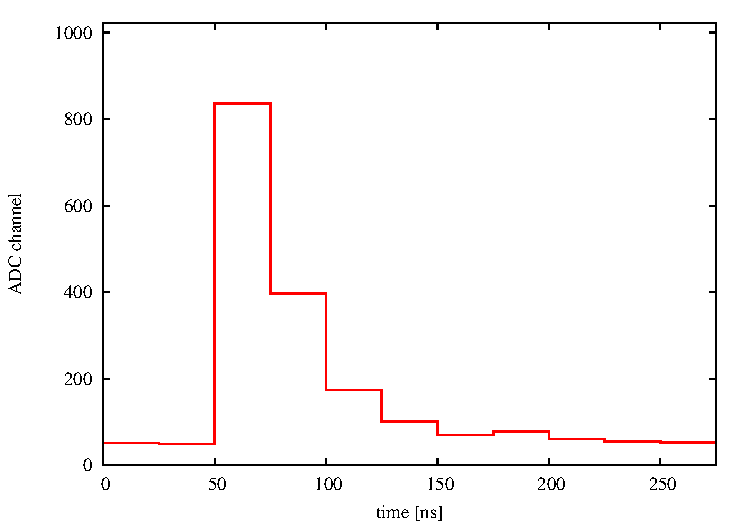
\includegraphics[width=0.6\textwidth]{images/bolivia/pulse.pdf}\\
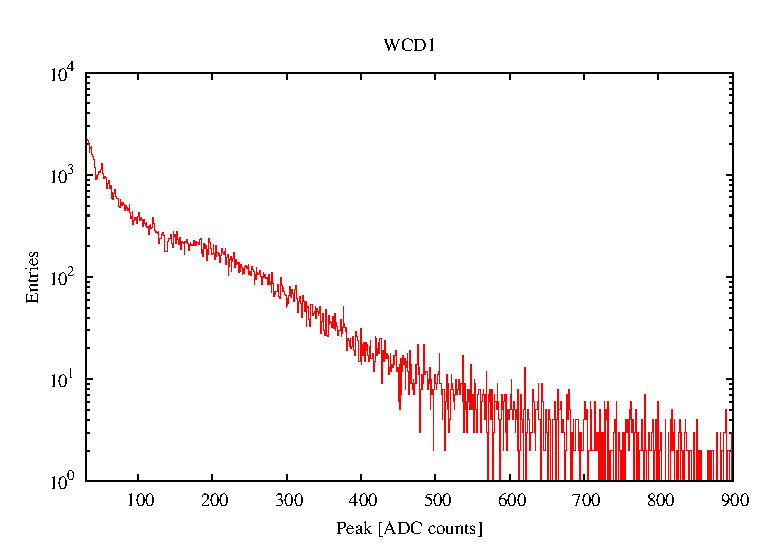
\includegraphics[width=0.49\textwidth]{images/bolivia/peakhist1.eps}
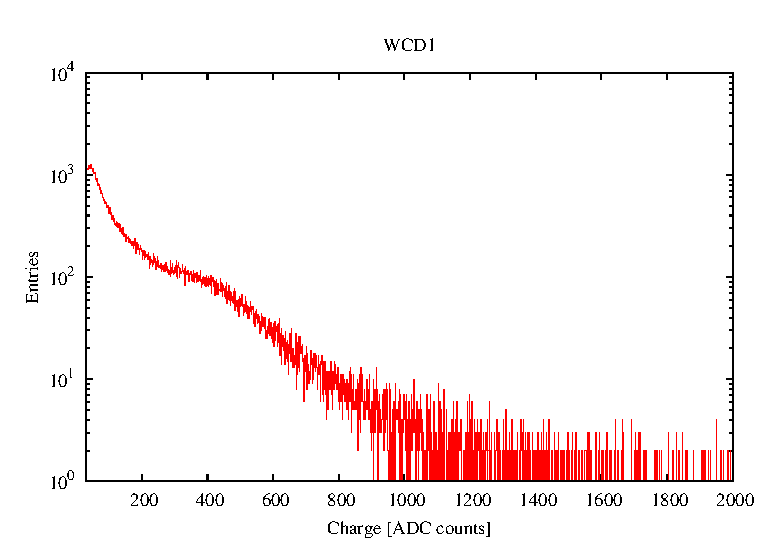
\includegraphics[width=0.49\textwidth]{images/bolivia/chargehist1.eps}
\end{center}
\caption{Top: A typical pulse shape obtained from a WCD. Bottom: Typical peak (left) and charge (right) histogram from one of the WCD located in mount Chacaltaya.}
\label{fig:bolivia-res}
\end{figure}

Two histograms are filled on a minute basis on each of the WCD. The first
histogram is filled with entries corresponding to the peaks (i.e. highest pulse
value) of the pulses received during a minute. The second histogram is filled
with entries corresponding to the charge (i.e. the integrated signal) of the
pulses. Two sample histograms are shown in figures \ref{fig:bolivia-res}, left
bottom and \ref{fig:bolivia-res}, right, corresponding to the WCD1. The muon
hump expected in the charge histogram is visible in the histogram, although not
as clearly as in a WCD located at sea level (see, for example, fig.
\ref{fig:bar-tanques} in section \ref{subsec:argen}. This is due to the
contribution of the electromagnetic component of showers (i. e. gamma rays and
electrons) which is dominant at very high altitudes.

As already noted, there are three WCD currently operational on the laboratory
at mount Chacaltaya and it is expected to have a new WCD operating at the
Higher University of San Simón in the near future, at the city of Cochabamba,
located on a valley with an elevation of almost 2600\,m.a.s.l.
